\subsection{GPU Accelerating Genotyping} \label{methods:gpu_accelerating_genotyping}
The genotyping step of KAGE (introduced in section \ref{background:kage}) computes genotype-probabilities, supported by the \textit{k}mer counts found during the \textit{k}mer counting portion.
A central part of this step is computing the \textit{logarithm of the probability mass function} (LOGPMF) a large number of times on large arrays.

The logarithm of the probability mass function at $k$ is computed using:
\begin{equation} \label{methods:gpu_accelerating_genotyping:equations:logpmf}
  logpmf = k * \log(\mu) - \mu - \ln(|\Gamma(k + 1)|)
\end{equation}
where $\Gamma$ is the gamma function.
In KAGE, this formula is computed for every element at index in two equal-sized arrays $k$ and $mu$.
The original implementation utilizes NumPy's efficient array-operations to compute LOGPMF efficiently using data-parallelism on the CPU.

\begin{figure}[H]
\begin{center}
\scalebox{.71}{
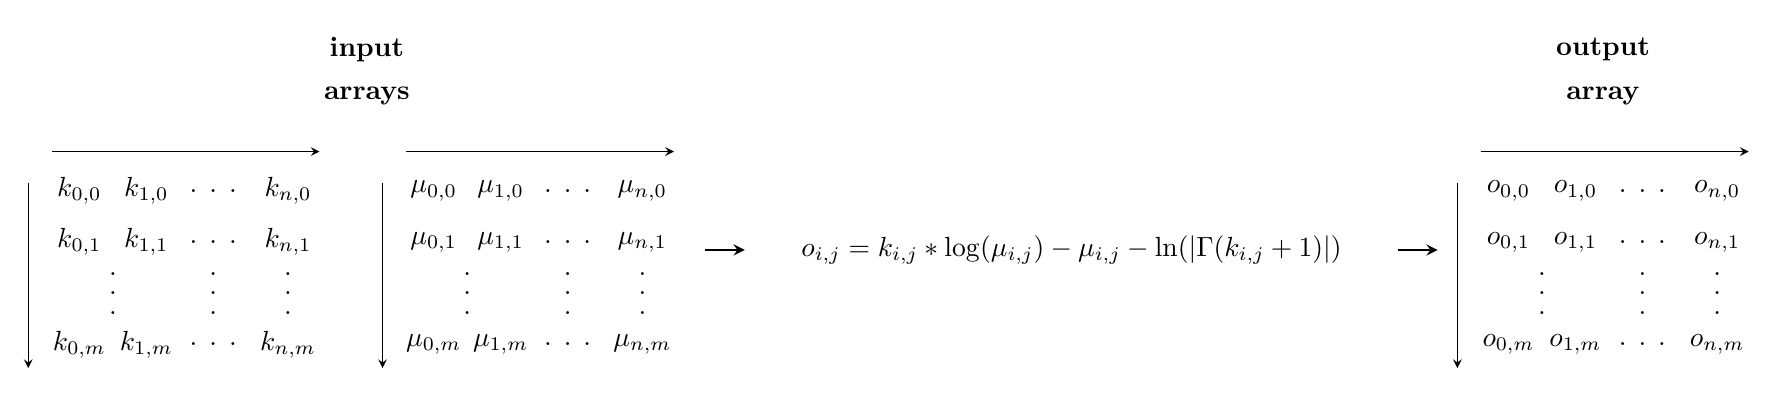
\begin{tikzpicture}
  % input
  \node at(2.9,3.8){\textbf{input}};
  \node at(2.9,3.2){\textbf{arrays}};
  % k
  \draw [-stealth](-1.1,2.5) -- (2.3,2.5);
  \draw [-stealth](-1.4,2.1) -- (-1.4,-.25);
  % row 0
  \node at(-.75,2){$k_{0,0}$};
  \node at(.1,2){$k_{1,0}$};
  \node at(.7,2){.};
  \node at(.95,2){.};
  \node at(1.2,2){.};
  \node at(1.9,2){$k_{n,0}$};
  % row 1
  \node at(-.75,1.35){$k_{0,1}$};
  \node at(.1,1.35){$k_{1,1}$};
  \node at(.7,1.35){.};
  \node at(.95,1.35){.};
  \node at(1.2,1.35){.};
  \node at(1.9,1.35){$k_{n,1}$};
  % dots
  % left
  \node at(-.325,.45){.};
  \node at(-.325,.7){.};
  \node at(-.325,.95){.};
  % middle 
  \node at(.95,.45){.};
  \node at(.95,.7){.};
  \node at(.95,.95){.};
  % right 
  \node at(1.9,.45){.};
  \node at(1.9,.7){.};
  \node at(1.9,.95){.};
  % row m
  \node at(-.75,.05){$k_{0,m}$};
  \node at(.1,.05){$k_{1,m}$};
  \node at(.7,.05){.};
  \node at(.95,.05){.};
  \node at(1.2,.05){.};
  \node at(1.9,.05){$k_{n,m}$};
  % mu
  \draw [-stealth](-1.1+4.5,2.5) -- (2.3+4.5,2.5);
  \draw [-stealth](-1.4+4.5,2.1) -- (-1.4+4.5,-.25);
  % row 0
  \node at(-.75+4.5,2){$\mu_{0,0}$};
  \node at(.1+4.5,2){$\mu_{1,0}$};
  \node at(.7+4.5,2){.};
  \node at(.95+4.5,2){.};
  \node at(1.2+4.5,2){.};
  \node at(1.9+4.5,2){$\mu_{n,0}$};
  % row 1
  \node at(-.75+4.5,1.35){$\mu_{0,1}$};
  \node at(.1+4.5,1.35){$\mu_{1,1}$};
  \node at(.7+4.5,1.35){.};
  \node at(.95+4.5,1.35){.};
  \node at(1.2+4.5,1.35){.};
  \node at(1.9+4.5,1.35){$\mu_{n,1}$};
  % dots
  % left
  \node at(-.325+4.5,.45){.};
  \node at(-.325+4.5,.7){.};
  \node at(-.325+4.5,.95){.};
  % middle 
  \node at(.95+4.5,.45){.};
  \node at(.95+4.5,.7){.};
  \node at(.95+4.5,.95){.};
  % right 
  \node at(1.9+4.5,.45){.};
  \node at(1.9+4.5,.7){.};
  \node at(1.9+4.5,.95){.};
  % row m
  \node at(-.75+4.5,.05){$\mu_{0,m}$};
  \node at(.1+4.5,.05){$\mu_{1,m}$};
  \node at(.7+4.5,.05){.};
  \node at(.95+4.5,.05){.};
  \node at(1.2+4.5,.05){.};
  \node at(1.9+4.5,.05){$\mu_{n,m}$};
  % arrow 1
  \draw [-stealth,thick](7.2,1.25) -- (7.7,1.25);
  % equation
  \node at(11.85,1.25){$o_{i,j}=k_{i,j}*\log(\mu_{i,j})-\mu_{i,j}-\ln(|\Gamma(k_{i,j}+1)|)$};
  % arrow 2
  \draw [-stealth,thick](16,1.25) -- (16.5,1.25);
  % output
  \node at(18.6,3.8){\textbf{output}};
  \node at(18.6,3.2){\textbf{array}};
  \draw [-stealth](-1.1+18.15,2.5) -- (2.3+18.15,2.5);
  \draw [-stealth](-1.4+18.15,2.1) -- (-1.4+18.15,-.25);
  % row 0
  \node at(-.75+18.15,2){$o_{0,0}$};
  \node at(.1+18.15,2){$o_{1,0}$};
  \node at(.7+18.15,2){.};
  \node at(.95+18.15,2){.};
  \node at(1.2+18.15,2){.};
  \node at(1.9+18.15,2){$o_{n,0}$};
  % row 1
  \node at(-.75+18.15,1.35){$o_{0,1}$};
  \node at(.1+18.15,1.35){$o_{1,1}$};
  \node at(.7+18.15,1.35){.};
  \node at(.95+18.15,1.35){.};
  \node at(1.2+18.15,1.35){.};
  \node at(1.9+18.15,1.35){$o_{n,1}$};
  % dots
  % left
  \node at(-.325+18.15,.45){.};
  \node at(-.325+18.15,.7){.};
  \node at(-.325+18.15,.95){.};
  % middle 
  \node at(.95+18.15,.45){.};
  \node at(.95+18.15,.7){.};
  \node at(.95+18.15,.95){.};
  % right 
  \node at(1.9+18.15,.45){.};
  \node at(1.9+18.15,.7){.};
  \node at(1.9+18.15,.95){.};
  % row m
  \node at(-.75+18.15,.05){$o_{0,m}$};
  \node at(.1+18.15,.05){$o_{1,m}$};
  \node at(.7+18.15,.05){.};
  \node at(.95+18.15,.05){.};
  \node at(1.2+18.15,.05){.};
  \node at(1.9+18.15,.05){$o_{n,m}$};
\end{tikzpicture}
}
\caption{
  The LOGPMF computation in KAGE is performed on large arrays, relying on NumPy's efficient and data-parallel solutions to run efficiently on the CPU.
}
\label{methods:gpu_accelerating_genotyping:figures:logpmf}
\end{center}
\end{figure}

\subsubsection{Replacing NumPy with CuPy}
Since the original KAGE solution for computing LOGPMF was implemented using NumPy, our first GPU acceleration was to use the method described in section \ref{methods:initial_testing:using_cupy_as_a_drop_in_replacement_for_numpy} where we used CuPy as a drop-in replacement for NumPy to GPU accelerate existing NumPy-based code.
The NumPy solution from KAGE relies on SciPy \cite{scipy} to compute the natural logarithm of the gamma function: $\ln(|\Gamma(x)|)$.
For our CuPy solution, we instead used CuPy's cupyx.scipy's implementation.

\begin{figure}[H] 
\begin{center}
logpmf.py
\end{center}
\begin{lstlisting}[language=Python,style=pycode]
import numpy as np
import cupy as cp

# Original function used in KAGE. Assumes k and r are NumPy arrays
def numpy_poisson_logpmf(k, r):
  return k * np.log(r) - r - scipy.special.gammaln(k+1) 

# Assumes k and r are CuPy arrays
def cupy_poisson_logpmf(k, r):
  return k * cp.log(r) - r - cupyx.scipy.special.gammaln(k+1) 
\end{lstlisting}
\caption{
  The original NumPy-based solution used in KAGE for computing LOGPMF, and a CuPy-based version for GPU acceleration.
  The CuPy-based GPU accelerated version assumes both input arrays, k and r, are residing in GPU memory.
}
\label{methods:gpu_accelerating_genotyping:figures:logpmf_array_implementations}
\end{figure}

\subsubsection{Assessment} \label{methods:gpu_accelerating_genotyping:cupy_logpmf_assessment}
In order to assess the effects of GPU accelerating KAGE's LOGPMF function by using CuPy, we benchmarked both functions by computing LOGPMF for input arrays $k$ and $r$.
The $k$ array was initialized with 40 million 32-bit integers, randomly set to values between 1 and 100.
$r$ was initialized with 40 million 64-bit floating point numbers, randomly set to values between 1 and 100.

The CuPy-based GPU accelerated function presented in figure \ref{methods:gpu_accelerating_genotyping:figures:logpmf_array_implementations} requires both input arrays, $k$ and $r$, to already be allocated in GPU memory.
Benchmarking only the function calls as presented therefore ignores the overhead of copying both $k$ and $r$ to GPU memory before the function call can be made.
Thus, for completion, we did not only benchmark both the NumPy and CuPy solutions. We additionally benchmarked the CuPy solution where $k$ and $r$ start off in CPU RAM and are copied to GPU memory before processing, and the result array is copied back to CPU RAM afterwards. 
This way, we accounted for the overhead of copying data to and from the GPU.

Our benchmarking yielded the following results:
\begin{table}[H]
\begin{center}
\begin{tabular}{lllll}
\multicolumn{1}{l|}{\textbf{Method}} & \multicolumn{1}{l}{\textbf{Time (milliseconds)}} &  \\ \cline{1-2}
\multicolumn{1}{l|}{NumPy} & \multicolumn{1}{l}{606.94} &  \\
\multicolumn{1}{l|}{CuPy (with copy)} & \multicolumn{1}{l}{201.9} & \\
\multicolumn{1}{l|}{CuPy (without copy)} & \multicolumn{1}{l}{82.49}
\end{tabular}
\end{center}
\caption{
  Time spent computing the logarithm of the probability mass function for 40 million elements.
  \textbf{NumPy} uses the NumPy-based solution with CPU data-parallelism and a single core.
  \textbf{CuPy (with copy)} uses the CuPy-based solution with GPU acceleration, but $k$ and $r$ are both copied from RAM to GPU memory before processing begins, and finally the result array is copied from GPU memory back to RAM.
  \textbf{CuPy (without copy)} uses the CuPy-based solution with GPU acceleration, but $k$ and $r$ are both already residing in GPU memory, and the result array is not copied back to RAM. In other words, we only measure the processing time of computing the 40 million LOGPMF values.
  Runtimes are the mean of 100 runs.
}
\label{methods:gpu_accelerating_genotyping:tables:logpmf_benchmark}
\end{table}

\begin{figure}[H]
\hspace*{7.25em}
\scalebox{.85}{
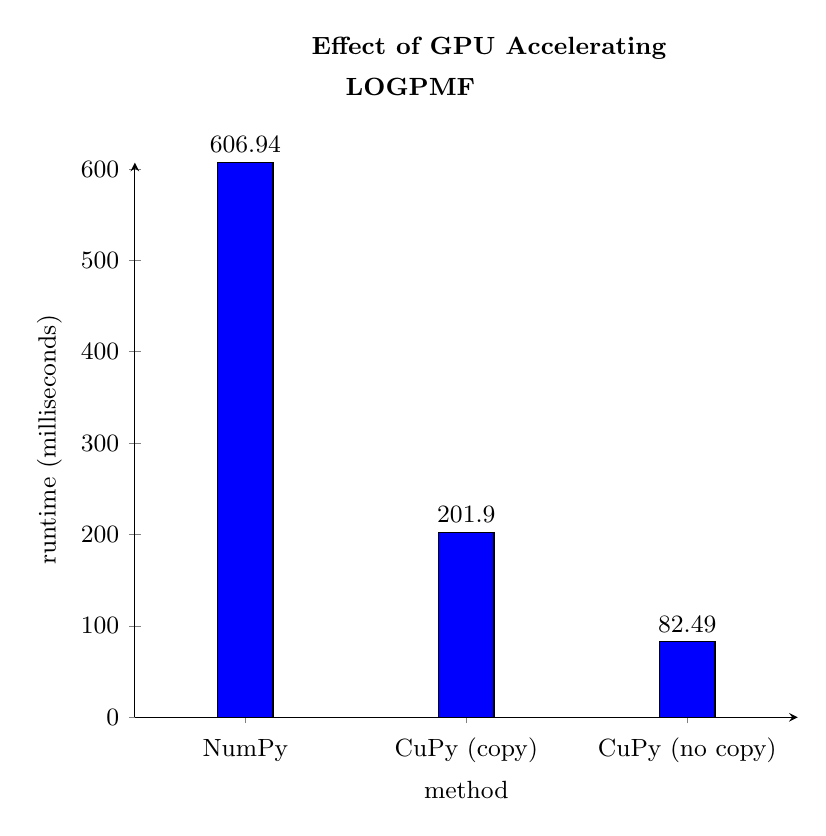
\begin{tikzpicture}[font=\small]
  \pgfplotsset{
    compat=newest,
    xlabel near ticks,
    ylabel near ticks
  }
  \pgfplotsset{compat=1.11,
      /pgfplots/ybar legend/.style={
      /pgfplots/legend image code/.code={%
         \draw[##1,/tikz/.cd,yshift=-0.25em]
          (0cm,0cm) rectangle (3pt,0.8em);},
     },
  }
  \node at(4.5,8.5)(){\textbf{Effect of GPU Accelerating}};
  \node at(3.5,8)(){\textbf{LOGPMF}};
 
\begin{axis} [
  ylabel={runtime (milliseconds)},
  xlabel={method},
  width=10cm,
  ybar,
  bar width=20pt,
  ymin=0,
  xtick=data,
  axis x line=bottom,
  axis y line=left,
  enlarge x limits=.25,
  symbolic x coords={NumPy, CuPy (copy), CuPy (no copy)},
  xticklabel style={anchor=base, yshift=-\baselineskip},
  /pgf/number format/.cd,fixed,precision=3,
  nodes near coords={\small\pgfmathprintnumber{\pgfplotspointmeta}},
  legend style={anchor=west},
]

\addplot[fill=blue] coordinates {
    (NumPy, 606.94)
    (CuPy (copy), 201.9)
    (CuPy (no copy), 82.49)
};
\end{axis}
\end{tikzpicture}
}
\caption{
  Time (milliseconds) spent computing the LOGPMF for input arrays of 40 million elements.
}
\label{methods:gpu_accelerating_genotyping:figures:logpmf_benchmark}
\end{figure}

\subsubsection{Implementing LOGPMF using CUDA}
While the method of using CuPy as a drop-in replacement for NumPy provided a significant speedup when computing the LOGPMF, it reveals a problem that arises when using NumPy and CuPy in Python.
When computing a nested expression, such as when computing the LOGPMF shown in equation \ref{methods:gpu_accelerating_genotyping:equations:logpmf}, the expression will be computed and evaluated following Python's evaluation rules, subsequently creating several temporary arrays.
This means that array allocations, de-allocations, memory writes and reads are happening needlessly while evaluating the Python expression.

By moving into C++ and using CUDA, we can create our own CUDA kernel to compute the LOGPMF for large arrays, avoiding these redundant operations.
We implemented a simple kernel where we avoid needlessly storing sub-expressions in temporary arrays.
\begin{figure}[H] 
\begin{center}
logpmf\_kernel.cu
\end{center}
\begin{lstlisting}[language=C++,style=cppcode]
__global__ void logpmf_kernel(
    const int *k, const double *r, double *out, const int size) {
  int i = blockIdx.x * blockDim.x + threadIdx.x;
  if (i < size) {
    out[i] = k[i] * logf(r[i]) - r[i] - lgammaf(k[i] + 1);
  }
}
\end{lstlisting}
\caption{
  The CUDA kernel implemented for computing the LOGPMF for arrays on the GPU.
}
\label{methods:gpu_accelerating_genotyping:figures:logpmf_kernel}
\end{figure}

\subsubsection{Assessment}
To benchmark the custom CUDA kernel we used the same benchmark as for the CuPy solution described in section \ref{methods:gpu_accelerating_genotyping:cupy_logpmf_assessment}.
Our benchmarking yielded the following results:
\begin{table}[H]
\begin{center}
\begin{tabular}{lllll}
\multicolumn{1}{l|}{\textbf{Method}} & \multicolumn{1}{l}{\textbf{Time (milliseconds)}} &  \\ \cline{1-2}
\multicolumn{1}{l|}{NumPy} & \multicolumn{1}{l}{606.94} &  \\
\multicolumn{1}{l|}{CuPy (with copy)} & \multicolumn{1}{l}{201.9} & \\
\multicolumn{1}{l|}{CuPy (without copy)} & \multicolumn{1}{l}{82.49} & \\
\multicolumn{1}{l|}{CUDA (with copy)} & \multicolumn{1}{l}{68.33} & \\
\multicolumn{1}{l|}{CUDA (without copy)} & \multicolumn{1}{l}{4.88}
\end{tabular}
\end{center}
\caption{
  Time spent computing the logarithm of the probability mass function for 40 million elements.
  \textbf{NumPy}, \textbf{CuPy (with copy)} and \textbf{CuPy (without copy)} are the benchmark results from table \ref{methods:gpu_accelerating_genotyping:tables:logpmf_benchmark}.
  \textbf{CUDA (with copy)} uses the custom CUDA kernel implementation, but $k$ and $r$ are both copied from RAM to GPU memory before the kernel is launched, and the result array is copied from GPU memory back to RAM.
  \textbf{CUDA (without copy)} uses the custom CUDA kernel implementation, but $k$ and $r$ are both already residing in GPU memory and the result array is not copied from GPU memory to RAM.
  Runtimes are the mean of 100 runs.
}
\label{methods:gpu_accelerating_genotyping:tables:logpmf_benchmark_2}
\end{table}

\begin{figure}[H]
\hspace*{2.75cm}
  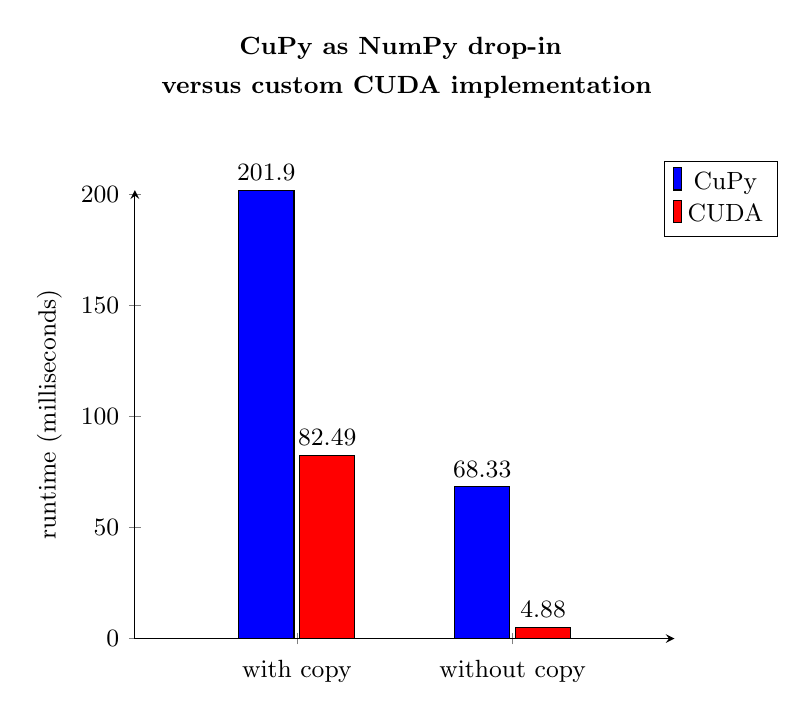
\begin{tikzpicture}[font=\small]
    \pgfplotsset{
      compat=newest,
      xlabel near ticks,
      ylabel near ticks
    }
    \pgfplotsset{compat=1.11,
        /pgfplots/ybar legend/.style={
        /pgfplots/legend image code/.code={%
           \draw[##1,/tikz/.cd,yshift=-0.25em]
            (0cm,0cm) rectangle (3pt,0.8em);},
       },
    }
    \node at(3.375,7.5)(){\small{\textbf{CuPy as NumPy drop-in}}};
    \node at(3.45,7)(){\small{\textbf{versus custom CUDA implementation}}};
 
\begin{axis} [
  ylabel={runtime (milliseconds)},
  ybar,
  bar width=20pt,
  ymin=0,
  xtick=data,
  axis x line=bottom,
  axis y line=left,
  enlarge x limits=0.75,
  symbolic x coords={with copy, without copy},
  xticklabel style={anchor=base, yshift=-\baselineskip},
  /pgf/number format/.cd,fixed,precision=3,
  nodes near coords={\small\pgfmathprintnumber{\pgfplotspointmeta}},
  every y tick scale label/.style={at={(yticklabel cs:1.1)},anchor=north},
  legend style={anchor=west},
]

\addplot[fill=blue] coordinates {
    (with copy, 201.9)
    (without copy, 68.33)
};

\addplot[fill=red] coordinates {
    (with copy, 82.49)
    (without copy, 4.88)
};
\legend{CuPy, CUDA}
\end{axis}
\end{tikzpicture}
\caption{
  Time (milliseconds) spent computing the LOGPMF for input arrays of 40 million elements.
}
\label{methods:gpu_accelerating_genotyping:figures:logpmf_benchmark_2}
\end{figure}

As can be seen in table \ref{methods:gpu_accelerating_genotyping:tables:logpmf_benchmark_2}, implementing our own CUDA solution, alleviating the wasteful array allocations and memory reads and writes, resulted in a significant speedup.

\subsubsection{Extending the LOGPMF Implementation}
...

\subsubsection{Assessment}
...
